\documentclass{beamer}
\usepackage[utf8]{inputenc}
\usepackage{verbatim}
\usepackage{clrscode}
\usepackage{multicol}
\setbeamertemplate{navigation symbols}{}
%\usetheme{Boadilla}
\setbeamertemplate{footline}[frame number]
\title{Algorithms for Longest Common Extensions}
\author{Jesper Kristensen}
\institute[DTU Informatics]{DTU Informatics\\Technical University of Denmark}
\date{August 31, 2011}
\begin{document}

\newcommand{\sortt}{\textit{sort}(n,\sigma)}
\newcommand{\LCE}{\textit{LCE}}
\newcommand{\NCA}{\textit{NCA}}
\newcommand{\RMQ}{\textit{RMQ}}
\newcommand{\SA}{\textit{SA}}
\newcommand{\SAinv}{\textit{SA}^{-1}} % math
\newcommand{\SAi}{SA$^{-1}$} % no math
\newcommand{\LCP}{\textit{LCP}}
\newcommand{\LA}{\textit{LA}}
\newcommand{\suff}{\textit{suff}}
\newcommand{\logceil}{\lceil\log n\rceil}
\newcommand{\fprint}[1][k]{\ensuremath{\proc{Fingerprint}_{#1}}}
\newcommand{\fprintk}{\fprint[k]}
\newcommand{\RMQpq}[2]{RMQ\textless$#1$, $#2$\textgreater}
\newcommand{\RMQn}{\RMQpq{1}{n}}
\newcommand{\RMQq}{\RMQpq{n}{1}}
\newcommand{\RMQlog}{\RMQpq{n}{\log n}}

\begin{frame}
\titlepage
\end{frame}

\begin{frame}{Contents}
\tableofcontents
\end{frame}

\section{Introduction}
\subsection{The LCE Problem}
\begin{frame}{The LCE Problem and the \proc{DirectComp} algorithm}
    \begin{block}{Input}
        \begin{itemize}
            \item $s=abbababba$
            \item $(i,j)=(4,6)$
        \end{itemize}
    \end{block}
    \begin{block}{The \proc{DirectComp} algorithm}
        %\setlength{\unitlength}{1cm}
        \definecolor{matchcolor}{rgb}{.6,1,.6}
        \definecolor{mismatchcolor}{rgb}{1,.6,.6}
        \begin{picture}(300,50)
            \put(0, 30){\makebox(20, 20){$s=$}}
            \put(20, 30){\framebox(20, 20){a}}
            \put(40, 30){\framebox(20, 20){b}}
            \put(60, 30){\framebox(20, 20){b}}
            \put(80, 30){\framebox(20, 20){a}}
            \put(100, 30){\framebox(20, 20){b}}
            \put(120, 30){\framebox(20, 20){a}}
            \put(140, 30){\framebox(20, 20){b}}
            \put(160, 30){\framebox(20, 20){b}}
            \put(180, 30){\framebox(20, 20){a}}
            \uncover<1-2>{
                \put(90, 15){\vector(0,1){13}}
                \put(80, 0){\makebox(20, 15){4}}
                \put(130, 15){\vector(0,1){13}}
                \put(120, 0){\makebox(20, 15){6}}
            }
            \uncover<2-2>{
                \put(80,30){\framebox(20, 20){\colorbox{matchcolor}{\makebox(13,14){a}}}}
                \put(120,30){\framebox(20, 20){\colorbox{matchcolor}{\makebox(13,14){a}}}}
            }
            \uncover<2-3>{
                \put(200, 30){\makebox(100, 20){1 match}}
            }
            \uncover<3-4>{
                \put(110, 15){\vector(0,1){13}}
                \put(100, 0){\makebox(20, 15){5}}
                \put(150, 15){\vector(0,1){13}}
                \put(140, 0){\makebox(20, 15){7}}
            }
            \uncover<4-4>{
                \put(100,30){\framebox(20, 20){\colorbox{matchcolor}{\makebox(13,14){b}}}}
                \put(140,30){\framebox(20, 20){\colorbox{matchcolor}{\makebox(13,14){b}}}}
            }
            \uncover<4->{
                \put(200, 30){\makebox(100, 20){2 matches}}
            }
            \uncover<5-6>{
                \put(130, 15){\vector(0,1){13}}
                \put(120, 0){\makebox(20, 15){6}}
                \put(170, 15){\vector(0,1){13}}
                \put(160, 0){\makebox(20, 15){8}}
            }
            \uncover<6-6>{
                \put(120,30){\framebox(20, 20){\colorbox{mismatchcolor}{\makebox(13,14){a}}}}
                \put(160,30){\framebox(20, 20){\colorbox{mismatchcolor}{\makebox(13,14){b}}}}
            }
        \end{picture}
    \end{block}
    \uncover<7->{
        \begin{block}{Result}
            $LCE_s(4,6)=2$
        \end{block}
        \begin{block}{LCE problem}
            Efficiently perform multiple queries $(i,j)$ on a static string $s$
        \end{block}
    }
\end{frame}

\subsection{The \proc{DirectComp} algorithm}
\begin{frame}{Existing Algorithm: \proc{DirectComp}}
    \begin{tabular}{r l}
        Preprocessing & $O(1)$ \\
        Space & $O(1)$ \\
        Query & $O(|\LCE(i,j)|)=O(n)$ \\
        Average query & $O(1)$ \\
        Query I/O & $O\Big(\frac{|\LCE(i,j)|}{B}\Big) = O\big(\frac{n}{B}\big)$ \\
    \end{tabular}

    \vspace{1cm}
    For a string length $n$ and alphabet size $\sigma$, the average LCE value over all $n^\sigma$ strings and $n^2$ query pairs is $O(1)$.
\end{frame}

\section{Existing Results}
%\subsection{The \proc{SuffixNca} Algorithm}
%\begin{frame}{Existing Algorithm: \proc{SuffixNca}}
%    $\LCE_s(i,j) = D[\NCA_\mathcal{T}(L_i,L_j)]$
%\end{frame}

\subsection{The \proc{LcpRmq} Algorithm}
\begin{frame}{Existing Algorithm: \proc{LcpRmq}}
    \begin{multicols}{2}{
        \begin{align*}
            s&=abbababba\\
            s[2\twodots n]&=bbababba\\
            s[3\twodots n]&=bababba\\
            \LCE_s(2,3)&=1
        \end{align*}
        \newpage
        \begin{center}
            %\uncover<2->{
            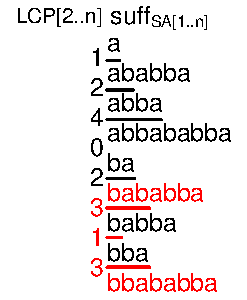
\includegraphics[width=0.26\textwidth,page=1]{../doc/sa+lcp+min.pdf}
            %}
        \end{center}
    }
    \end{multicols}
    %\uncover<3->{
    \begin{center}
        $\LCE(i,j)=\LCP[\RMQ_{\LCP}(\SAinv[i] + 1, \SAinv[j])]$\\
        where $\SAinv[i] < \SAinv[j]$\\
        \vspace{1em}
        \begin{tabular}{r l}
            Preprocessing & $O(\sortt)$ \\
            Space & $O(n)$ \\
            Query & $O(1)$ \\
            Average query & $O(1)$ \\
            Query I/O & $O(1)$ \\
        \end{tabular}
    \end{center}
    %}
\end{frame}

\subsection{Practical results}
\begin{frame}{Existing Algorithms: Practical Results}
    Query times of
    \textcolor{red}{\proc{DirectComp}} and
    \textcolor{green}{\proc{LcpRmq}}
    by string length
    \begin{multicols}{2}{
        \begin{center}
            Average case
            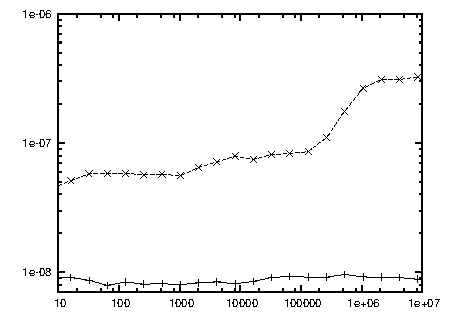
\includegraphics[width=0.49\textwidth,type=pdf,ext=.pdf,read=.pdf]{../src/results/length-rmq-directcomp-slide-rand10.plt}
            \newpage
            Worst case
            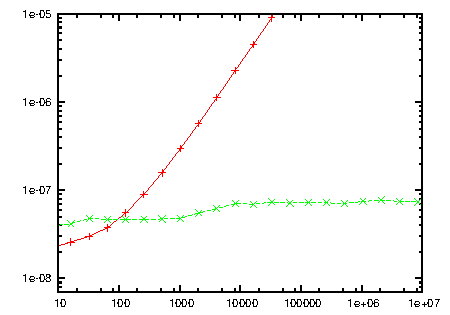
\includegraphics[width=0.49\textwidth,type=pdf,ext=.pdf,read=.pdf]{../src/results/length-rmq-directcomp-slide-alla.plt}
        \end{center}
    }
    \end{multicols}

\end{frame}

\section{The \fprintk\ Algorithm}
\subsection{Data Structure}
\begin{frame}{The \fprintk\ Algorithm: Data Structure}
    \begin{itemize}
        \item For a string $s[1\twodots n]$, the $t$-length fingerprints $F_t[1\twodots n]$ are natural numbers, such that $F_t[i] = F_t[j]$ if and only if $s[i\twodots i+t-1] = s[j\twodots j+t-1]$.
        \item $k$ levels, $1\leq k\leq\logceil$
        \item For each level, $\ell = 0\twodots k-1$:
        \begin{itemize}
            \item $t_\ell = \Theta(n^{\ell/k}), t_0=1$
            \item $H_\ell = F_{t_\ell}$
        \end{itemize}
    \end{itemize}
    \begin{center}
        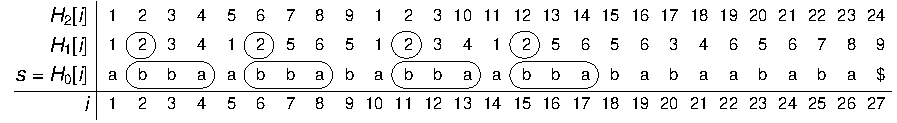
\includegraphics[width=1\textwidth,page=1]{../doc/fingerprint.pdf}
    \end{center}
    \begin{tabular}{r l}
        Space & $O(k\cdot n)$\\
    \end{tabular}
\end{frame}

\subsection{Query}
\begin{frame}{The \fprintk\ Algorithm: Query}
    \begin{enumerate}
        \item As long as $H_\ell[i+v] = H_\ell[j+v]$, increment $v$ by $t_\ell$, increment $\ell$ by one, and repeat this step unless and $\ell = k-1$.
        \item As long as $H_\ell[i+v] = H_\ell[j+v]$, increment $v$ by $t_\ell$ and repeat this step.
        \item Stop and return $v$ when $\ell = 0$, otherwise decrement $\ell$ by one and go to step two.
    \end{enumerate}
    \begin{center}
        \includegraphics[width=1\textwidth,page=2]{../doc/fingerprint.pdf}\\
         $\LCE(3,12)=9$
    \end{center}
    \begin{tabular}{r l}
        Query & $O(k\cdot n^{1/k})$ \\
        Average query & $O(1)$ \\
    \end{tabular}
\end{frame}

\subsection{Preprocessing}
\begin{frame}{The \fprintk\ Algorithm: Preprocessing}
    \begin{itemize}
        \item For each level $\ell$
        \begin{itemize}
            \item For each $t_\ell$-length substring in lexicographically sorted order
            \begin{itemize}
                \item If the current substring $s[\SA[i]\twodots\SA[i]+t_\ell-1]$ is equal to the previous substring, give it the same fingerprint as the previous substring, otherwise give it a new unused fingerprint. The two substrings are equal when $\LCE[i] \geq t_\ell$.
            \end{itemize}
        \end{itemize}
    \end{itemize}

    \begin{multicols}{2}{
        \begin{center}
        \hfill\\
            $s=$ abbababba\\\hfill\\
            For $t_\ell = 3$:\\
            $H_\ell =$ [3, 8, 6, 2, 6, 3, 8, 5, 1]
        \end{center}
        \newpage
        \begin{center}
            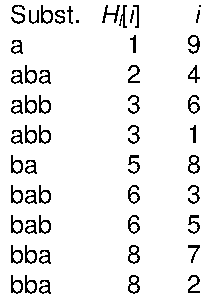
\includegraphics[width=0.2\textwidth,page=1]{../doc/fingerprint-preproc.pdf}
        \end{center}
    }
    \end{multicols}

    \begin{tabular}{r l}
        Preprocessing & $O(k\cdot n + \sortt)$ \\
    \end{tabular}

\end{frame}

\subsection{I/O}
\begin{frame}{The \fprintk\ Algorithm: I/O}
    \begin{itemize}
        \item Original:
        \begin{itemize}
            \item Data structure: $H_\ell[i] = F_{t_\ell}[i]$
            \item Size: $|H_\ell| = n$
            \item I/O: $O\big(k\cdot n^{1/k}\big)$
        \end{itemize}
        \item Cache optimized:
        %Instead of storing the fingerprint of $s[i\twodots i+t_\ell-1]$ at $H_\ell[i]$, we can store it at 
        \begin{itemize}
            \item Data structure: \\~~$H_\ell[((i-1)\mod t_\ell)\cdot\lceil n/t_\ell\rceil+\lfloor (i-1)/t_\ell\rfloor+1] = F_{t_\ell}[i]$
            \item Size: $|H_\ell| = n+t_\ell$
            \item I/O: $O\Big(k\cdot\Big(\frac{n^{1/k}}{B}+1\Big)\Big)$
            \begin{itemize}
                \item Best when $k$ is small $\implies$ $n^{1/k}$ is large.
            \end{itemize}
        \end{itemize}
     \end{itemize}
     %$n+t_\ell-1/t_\ell+2$
    \begin{center}
        \includegraphics[width=0.7\textwidth,page=2]{../doc/fingerprint.pdf}\\
    \end{center}
\end{frame}

\begin{frame}{The \fprintk\ Algorithm}
    \begin{tabular}{r l}
        Preprocessing & $O(k\cdot n + \sortt)$ \\
        Space & $O(k\cdot n)$\\
        Query & $O(k\cdot n^{1/k})$ \\
        Average query & $O(1)$ \\
        Query I/O & $O\Big(k\cdot\Big(\frac{n^{1/k}}{B}+1\Big)\Big)$ \\
    \end{tabular}

    \hfill\\$k=1$:

    ~~Same as \proc{DirectComp}

%    \hfill\\$k=2$:

%    \begin{tabular}{r l}
%        Preprocessing & $O(\sortt)$ \\
%        Space & $O(n)$\\
%        Query & $O(\sqrt n)$ \\
%        Average query & $O(1)$ \\
%    \end{tabular}

    \begin{multicols}{2}{
        $k=2$:

        \begin{tabular}{r l}
            Preprocessing & $O(\sortt)$ \\
            Space & $O(n)$\\
            Query & $O(\sqrt n)$ \\
            Average query & $O(1)$ \\
            Query I/O & $O\Big(\frac{\sqrt n}{B}\Big)$ \\
        \end{tabular}
        \newpage
        $k=\logceil$:

        \begin{tabular}{r l}
            Preprocessing & $O(n\log n)$ \\
            Space & $O(n\log n)$\\
            Query & $O(\log n)$ \\
            Average query & $O(1)$ \\
            Query I/O & $O(\log n)$ \\
        \end{tabular}
    }
    \end{multicols}
\end{frame}

\subsection{Practical Results}
\begin{frame}{Practical Results}
    Query times of
    \textcolor{red}{\proc{DirectComp}},
    \textcolor{green}{\fprint[2] (cache opt.)},
    \textcolor{blue}{\fprint[3] (not cache opt.)},
    \textcolor{magenta}{\fprint[\logceil] (not cache opt.)} and
    \textcolor{cyan}{\proc{LcpRmq}}
    by string length
    \begin{multicols}{2}{
        \begin{center}
            Average case
            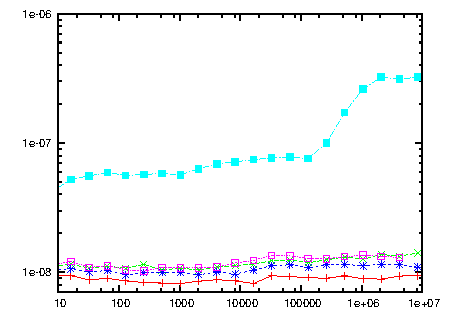
\includegraphics[width=0.49\textwidth,type=pdf,ext=.pdf,read=.pdf]{../src/results/length-slides-cache-rand10.plt}
            \newpage
            Worst case
            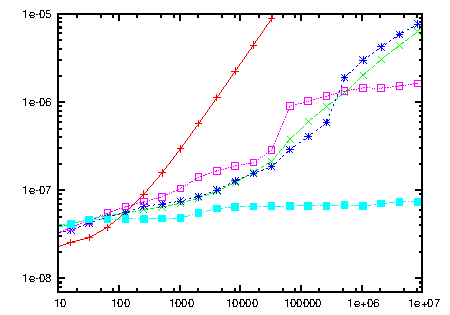
\includegraphics[width=0.49\textwidth,type=pdf,ext=.pdf,read=.pdf]{../src/results/length-slides-cache-alla.plt}
        \end{center}
    }
    \end{multicols}
\end {frame}

\begin{frame}{Practical Results}
    Query times of
    \textcolor{red}{\proc{DirectComp}},
    \textcolor{green}{\fprint[2] (cache opt.)},
    \textcolor{blue}{\fprint[3] (not cache opt.)},
    \textcolor{magenta}{\fprint[\logceil] (not cache opt.)} and
    \textcolor{cyan}{\proc{LcpRmq}}
    by string length
    \begin{center}
        Medium LCE size\\
        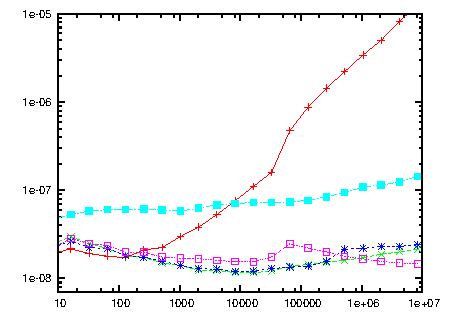
\includegraphics[width=0.49\textwidth,type=pdf,ext=.pdf,read=.pdf]{../src/results/length-slides-cache-repeat-pow.plt}
    \end{center}
\end {frame}

\begin{frame}{Cache Optimization, Practical Results}
    Is I/O optimization good in practice?
    \begin{itemize}
        \item Pro: better cache efficiency
            \begin{itemize}
                \item Best for small $k$, no change for $k=\logceil$
            \end{itemize}
        \item Con: Calculating memory addresses is more complicated
            \begin{itemize}
                \item $((i-1)\mod t_\ell)\cdot\lceil n/t_\ell\rceil+\lfloor (i-1)/t_\ell\rfloor+1$ vs.\ $i$
            \end{itemize}
    \end{itemize}
\end{frame}

%\subsection{Practical I/O}
\begin{frame}{The \fprintk\ Algorithm: Practical Results, I/O}
    Query times of \fprint[2]
    \textcolor{red}{without cache optimization}
    and with cache optimization using
    \textcolor{green}{shift operations} vs.\
    \textcolor{blue}{multiplication and division}
    %by string length
    \begin{multicols}{2}{
        \begin{center}
            Average case
            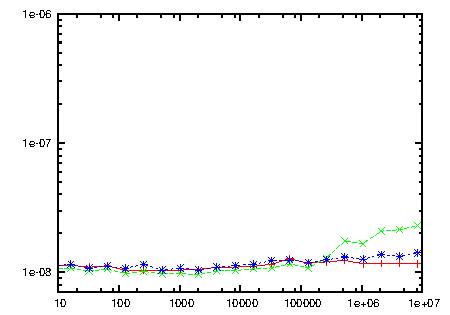
\includegraphics[width=0.49\textwidth,type=pdf,ext=.pdf,read=.pdf]{../src/results/length-slides-cache-fp2-rand10.plt}
            \newpage
            Worst case
            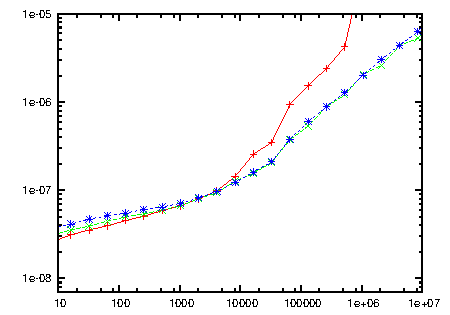
\includegraphics[width=0.49\textwidth,type=pdf,ext=.pdf,read=.pdf]{../src/results/length-slides-cache-fp2-alla.plt}
        \end{center}
    }
    \end{multicols}
\end{frame}

\begin{frame}{The \fprintk\ Algorithm: Practical Results, I/O}
    Query times of \fprint[3]
    \textcolor{red}{without cache optimization}
    and with cache optimization using
    \textcolor{green}{shift operations} vs.\
    \textcolor{blue}{multiplication and division}
    %by string length
    \begin{multicols}{2}{
        \begin{center}
            Average case
            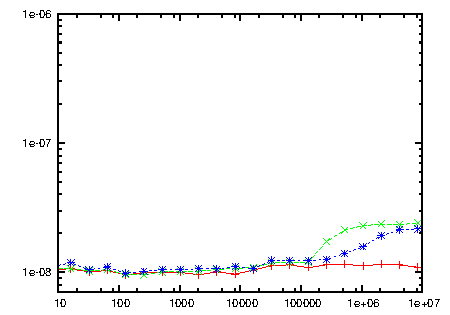
\includegraphics[width=0.49\textwidth,type=pdf,ext=.pdf,read=.pdf]{../src/results/length-slides-cache-fp3-rand10.plt}
            \newpage
            Worst case
            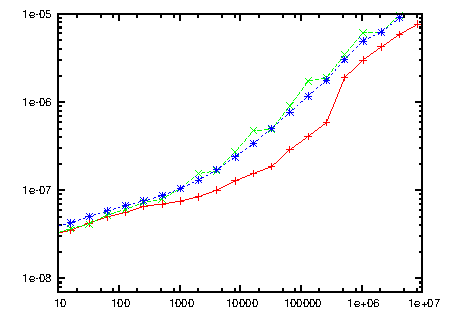
\includegraphics[width=0.49\textwidth,type=pdf,ext=.pdf,read=.pdf]{../src/results/length-slides-cache-fp3-alla.plt}
        \end{center}
    }
    \end{multicols}
\end{frame}

\begin{frame}{The \fprintk\ Algorithm: Practical Results, I/O}
    Query times of
    \textcolor{red}{\proc{DirectComp}},
    \textcolor{green}{\fprint[2] (cache opt.)},
    \textcolor{blue}{\fprint[3] (not cache opt.)},
    \textcolor{magenta}{\fprint[\logceil] (not cache opt.)} and
    \textcolor{cyan}{\proc{LcpRmq}}
    by string length
    \begin{multicols}{2}{
        \begin{center}
            Average case
            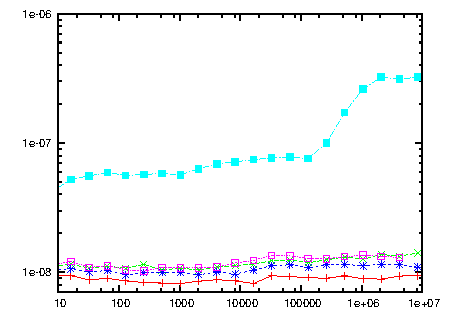
\includegraphics[width=0.49\textwidth,type=pdf,ext=.pdf,read=.pdf]{../src/results/length-slides-cache-rand10.plt}
            \newpage
            Cache stress\\
            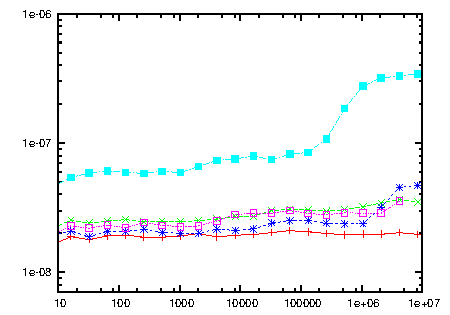
\includegraphics[width=0.49\textwidth,type=pdf,ext=.pdf,read=.pdf]{../src/results/length-slides-cache-rand2.plt}
        \end{center}
    }
    \end{multicols}
\end {frame}

\begin{comment}
\section{LCE on trees}
\subsection{Compression}
\begin{frame}{LCE on Compressed Strings}
    Goal
    \begin{itemize}
        \item Allow LCE queries without decompressing the string
        \item Using Ziv-Lempel compression (LZ)
    \end{itemize}
    How
    \begin{itemize}
        \item LZ compression represents the string as a tree
        \item An LCE query on a LZ compressed string is a number of LCE queries on a tree
    \end{itemize}
\end{frame}

\begin{frame}{LCE on Trees}
    \begin{itemize}
        \item Trees:
        \begin{itemize}
            \item One character on each edge
            \item LCE is the length of the longest common prefix of two strings along two paths
        \end{itemize}
        \item $p_i=bbc$ and $p_j=bbba$ gives $\LCE(p_i,p_j)=2$
    \end{itemize}
    \begin{center}
        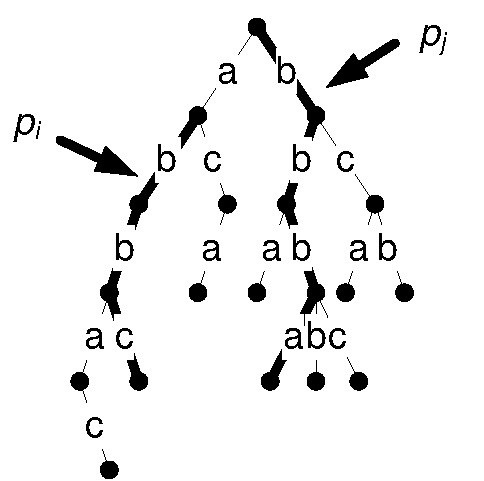
\includegraphics[width=0.4\textwidth,page=1]{tree-lce.pdf}
    \end{center}
\end{frame}

\subsection{Constant Time String LCE on Heavy Paths}
\begin{frame}{Constant Time String LCE on Heavy Paths}
    \begin{multicols}{2}{
        \begin{itemize}
            \item Data structure:
            \begin{itemize}
                \item Construct a heavy tree decomposition
                \item For each heavy path, store characters as a substring
            \end{itemize}
            \item Query:
            \begin{itemize}
                \item Use constant time string LCE on each heavy path
            \end{itemize}
        \end{itemize}
        \begin{center}
            \includegraphics[width=0.44\textwidth,page=4]{../doc/tree-fingerprint.pdf}
        \end{center}
        \begin{tabular}{r l}
            Preprocessing & $O(\sortt)$ \\
            Space & $O(n)$\\
            Query & $O(\log n)$ \\
        \end{tabular}
    }
    \end{multicols}
\end{frame}

\begin{frame}{Constant Time String LCE on Heavy Paths}
    \begin{columns}[t]
        \begin{column}{0.7\textwidth}
            \begin{itemize}
                \item How to find the indexes $(i,j)$ in the string:
                \begin{itemize}
                    \item Store an index at each node
                \end{itemize}
                \item How to know then the heavy path splits from the queried path:
                \begin{itemize}
                    \item Store a pointer to the end of the heavy path at each node
                    \item Find NCA of the end of the heavy path and the end of the queried path
                \end{itemize}
                \item How to find a node on the queried path:
                \begin{itemize}
                    \item Use level ancestor
                \end{itemize}
            \end{itemize}
        \end{column}
        \begin{column}{0.3\textwidth}
        \hfill\\
            \includegraphics[width=1\textwidth,page=3]{../doc/tree-fingerprint.pdf}
        \end{column}
    \end{columns}
\end{frame}
\end{comment}

\section{Summary}
\begin{frame}{Summary}
    \begin{tabular}{r l l l}
        & \proc{Direct-} & \proc{LcpRmq} / & \\
        & \proc{Comp} & \proc{SuffixNca} & \fprintk \\
        Preprocessing & $O(1)$ & $O(\sortt)$ & $O(k\cdot n+\sortt)$ \\
        Space & $O(1)$ & $O(n)$ & $O(k\cdot n)$\\
        Query & $O(n)$ & $O(1)$ & $O(k\cdot n^{1/k})$ \\
        Average query & $O(1)$ & $O(1)$ & $O(1)$ \\
        Query I/O & $O\big(\frac{n}{B}\big)$ & $O(1)$ & $O\Big(k\cdot\Big(\frac{n^{1/k}}{B}+1\Big)\Big)$ \\
    \end{tabular}
    \vspace{1em}
    \begin{itemize}
        \item In practice, the \fprintk\ algorithm is...
        \begin{itemize}
            \item ...almost as good as \proc{DirectComp} and significantly better than \proc{LcpRmq} in average case
            \item ...significantly better than \proc{DirectComp} but worse than \proc{LcpRmq} in worst case
        \end{itemize}
        \item Cache optimization of \fprintk\ improves query times at $k=2$ and worsens query times at $k\geq 3$
        %\item We can generalize LCE to use on trees:
        %\begin{tabular}{r l}
        %    Preprocessing & $O(\sortt)$ \\
        %    Space & $O(n)$\\
        %    Query & $O(\log n)$ \\
        %\end{tabular}
    \end{itemize}
\end {frame}

\end{document}






















